\documentclass[12pt]{article}

\usepackage[margin=1cm, paperheight=60in]{geometry}
\usepackage{amsfonts, multicol, pgfplots, tikz}

\pgfplotsset{compat=1.18}
\title{Section 2 homework}
\author{Michael Padilla}

\begin{document}
\maketitle

\section*{Exercises for Section 2.1}
\begin{itemize}
    \item[A.] Write each of the following sets by listing their elements between braces.
	\begin{enumerate}
	    \item $\{5x - 1 : x \in \mathbb{Z}\} = \{\ldots, -11, -6, -1, 4, 9, \ldots\}$
	    \item $\{3x + 2 : x \in \mathbb{Z}\} = \{\ldots, -4, -1, 2, 5, 8, \ldots\}$
	    \item $\{x \in \mathbb{Z} : -2 \le x < 7\} = \{-2, -1, 0, 1, 2, 3, 4, 5, 6\}$
	    \item $\{x \in \mathbb{N} : -2 < x \le 7\} = \{1, 2, 3, 4, 5, 6, 7 \}$
	    \item $\{x \in \mathbb{R} : x^2 = 3\} = \{-\sqrt{3}, \sqrt{3}  \}$
	    \item $\{x \in \mathbb{R} : x^2 = 9\} = \{-3, 3  \}$
	    \item $\{x \in \mathbb{R} : x^2 + 5x = -6\} = \{-3, -2  \}$
	    \item[11] $\{x \in \mathbb{Z} : |x| < 5 \} = \{-4, -3, -2, -1, 0, 1, 2, 3, 4  \}$
	    \item[12] $\{x \in \mathbb{Z} : |2x| < 5 \} = \{-2, -1, 0, 1, 2 \}$
	    \item[13] $\{x \in \mathbb{Z} : |6x| < 5 \} = \{0\}$
	    \item[14] $\{5x : x \in \mathbb{Z}, |2x| \le 8 \} = \{-20, -15, -10, -5, 0, 5, 10, 15, 20 \}$
	\end{enumerate}
    \item[B.] Write each of the following sets in set-builder notation.
	\begin{enumerate}
	    \item[17] $\{2,4,8,16,32,64\ldots\} = \{2 \cdot 2^x: x \ge 0, x \in \mathbb{Z}\}$
	    \item[19] $\{\ldots, -6, -3, 0, 3, 6, 9, 12, 15, \ldots \} = \{3x: x \in \mathbb{Z}\}$
	    \item[24] $\{-4,-3,-2,-1,-0,1,2\} = \{x: -4 \le x \le 2, x \in \mathbb{Z}\}$
	    \item[25] $\{\ldots, \frac{1}{8} ,\frac{1}{4} ,\frac{1}{2},1,2,4,8, \ldots\} = \{2^x:x \in \mathbb{Z}\}$
	    \item[26] $\{\ldots, \frac{1}{27} ,\frac{1}{9},\frac{1}{3},1,3,9,27, \ldots\} = \{3^x:x \in \mathbb{Z}\}$
	\end{enumerate}
    \item[C.] Find the following cardinalities of the following sets.
	\begin{multicols}{2}
	\begin{enumerate}
	    \item[29] $\{\{1\}, \{2, \{3, 4\}\}, \phi\} = 3$
	    \item[30] $\{\{1,4\}, a, b, \{\{3, 4\}\}, \{\phi\}\} = 5$
	    \item[31] $\{\{\{1\}, \{2, \{3,4\}\}, \phi\}\} = 1$
	    \item[32] $\{\{\{1,4\}, a,b, \{\{3,4\}\}, \{\phi\}\}\} = 1$
	    \item[33] $\{x \in \mathbb{Z} : |x| < 10\} = 19$
	    \item[34] $\{x \in \mathbb{N} : |x| < 10\} = 9$
	    \item[35] $\{x \in \mathbb{Z} : x^2 < 10\} = 7$
	    \item[36] $\{x \in \mathbb{N} : x^2 < 10\} = 3$
	    \item[37] $\{x \in \mathbb{N} : x^2 < 0\} = 0$
	    \item[38] $\{x \in \mathbb{N} : 5x \le 20\} = 4$
	\end{enumerate}
	\end{multicols}
\end{itemize}
\section*{Exercises for Section 2.2}
\begin{itemize}
    \item [A] Write out the indicated sets by listing their elements between braces.
	\begin{itemize}
	    \item [2] Suppose $A=\{\pi, e, 0\}$ and $B=\{0,1\}$.
		\begin{itemize}
		    \item $A \times B = \{(\pi, 0), (\pi, 1), (e, 0), (e, 1), (0, 0), (0, 1)\}$
		    \item $B \times A = \{(0, \pi),(0, e), (0, 0), (1, \pi), (1, e), (1, 0)\}$
		    \item $A \times A = $\\
		    $\{(\pi, \pi), (\pi, e), (\pi, 0), (e, \pi), (e, e), (e, 0), (0, \pi), (0, e), (0, 0)\}$
		    \item $B \times B = \{ (0, 0), (0, 1), (1, 0), (1, 1)\}$
		    \item $A \times \phi = \{(\pi), (e), (0)\}$
		    \item $(A \times B) \times B = $\\
		    $\{((\pi, 0), 0), ((\pi, 0), 1), ((\pi, 1), 0), ((\pi, 1), 1), ((e, 0), 0), ((e, 0), 1),$\\
		    $((e, 1), 0), ((e, 1), 1), ((0, 0), 0), ((0, 0), 1), ((0, 1), 0), ((0, 1), 1)\}$
		    \item $A \times (B \times B) = $\\
		    $\{ (\pi,(0, 0)), (\pi, (0, 1)), (\pi, (1, 0)), (\pi,(1, 1)),$\\
		    $(e,(0, 0)), (e, (0, 1)), (e, (1, 0)), (e,(1, 1)),$\\
		    $(0,(0, 0)), (0, (0, 1)), (0, (1, 0)), (0,(1, 1))\}$
		    \item $A \times B \times B =$\\
			$\{(\pi, 0, 0), (\pi, 0, 1), (\pi, 1, 0), (\pi, 1, 1),$\\
			$(e, 0, 0), (e, 0, 1), (e, 1, 0), (e, 1, 1),$\\
			$(0, 0, 0), (0, 0, 1), (0, 1, 0), (0, 1, 1)\}$
		\end{itemize}
	    \item [6] $\{x \in \mathbb{R} : x^2 = x\} \times \{x \in \mathbb{N} : x^2 = x\} = \{(0, 1), (1, 1)\}$
	    \item [8] $\{0, 1 \}^4 =$\\
	    $\{(((0, 0), 0), 0), (((0,0), 0), 1), (((0, 0), 1), 0), (((0,0), 1), 1), (((0, 1), 0),0),$\\
	    $(((0,1), 0), 1), (((0, 1), 1), 0), (((0,1),1),1), (((1, 0), 0), 0), (((1,0), 0), 1),$\\
	    $(((1, 0), 1),0), (((1,0), 1), 1), (((1, 1), 0), 0), (((1,1), 0), 1),$\\
	    $(((1, 1), 1), 0), (((1,1),1),1)\}$
	\end{itemize}
    \item [B] Sketch these Cartesian products on the $x-y$ plane $\mathbb{R}^2$ (or $\mathbb{R}^3$for the last two.)
	\begin{itemize}
	    \item [9] $\{1,2,3\} \times \{-1,0,1\} = \{(1, -1), (1, 0), (1, 1), (2, -1), (2, 0), (2, 1), (3, -1), (3, 0), (3, 1)\}$\\
		\begin{tikzpicture}
		    \begin{axis}[xmin=0, xmax=4, ymin=-2, ymax=2, axis lines=middle]
			\addplot[mark=*] coordinates {(1,-1)};
			\addplot[mark=*] coordinates {(1,0)};
			\addplot[mark=*] coordinates {(1,1)};
			\addplot[mark=*] coordinates {(2,-1)};
			\addplot[mark=*] coordinates {(2,0)};
			\addplot[mark=*] coordinates {(2,1)};
			\addplot[mark=*] coordinates {(3,-1)};
			\addplot[mark=*] coordinates {(3,0)};
			\addplot[mark=*] coordinates {(3,1)};
		    \end{axis}
		\end{tikzpicture}
	    \item [11] $[0,1]\times [0,1]$\\
		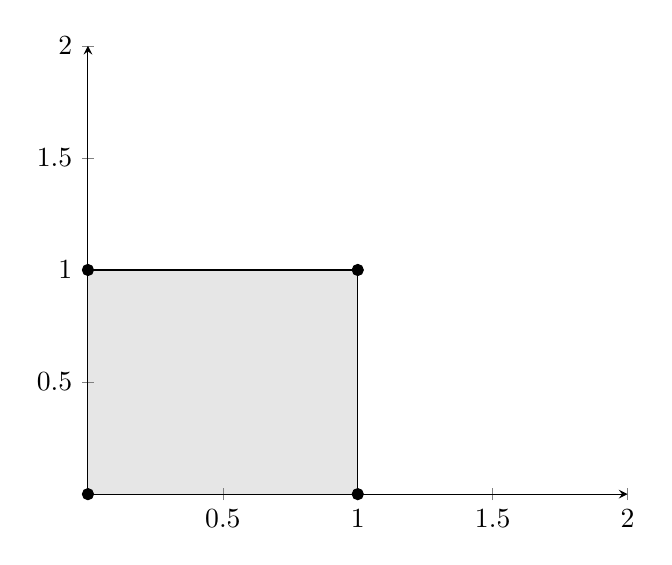
\begin{tikzpicture}
		    \begin{axis}[xmin=0, xmax=2, ymin=0, ymax=2, axis lines=middle]
			\addplot [mark=*,mark options={fill=black, fill opacity=1},fill=gray,fill opacity=0.2] coordinates {(0,0) (1,0) (1,1) (0,1)};
		    \end{axis}
		\end{tikzpicture}
	    \item [13] $\{1,1.5,2\}\times[1,2]$\\
		\begin{tikzpicture}
		    \begin{axis}[xmin=0, xmax=3, ymin=0, ymax=3, axis lines=middle]
			\addplot [mark=*] coordinates {(1,1) (1,2)};
			\addplot [mark=*] coordinates {(1.5,1) (1.5,2)};
			\addplot [mark=*] coordinates {(2,1) (2,2)};
		    \end{axis}
		\end{tikzpicture}
	    \item [15] $\{1\}\times[0,1]$\\
		\begin{tikzpicture}
		    \begin{axis}[xmin=0, xmax=2, ymin=0, ymax=2, axis lines=middle]
			\addplot [mark=*] coordinates {(1,0) (1,1)};
		    \end{axis}
		\end{tikzpicture}
	\end{itemize}
\end{itemize}
\section*{Exercises for Section 2.3}
    \begin{itemize}
	\item [A] List all the subsets of the following sets.
	    \begin{enumerate}
		\item $\{1,2,3,4\} = \{\}, \{1\}, \{2\}, \{3\}, \{4\}, \{1,2\},\{1,3\},\{1,4\},$\\
		    $\{2,3\}, \{2,4\}, \{3,4\}, \{1,2,3\}, \{1,2,4\}, \{1,3,4\}, \{2,3,4\}, \{1,2,3,4\} $
		\item $\{1,2,\phi\} = \{\}, \{1\}, \{2\}, \{\phi\}, \{1,2\}, \{1,\phi\}, \{2,\phi\}, \{1,2,\phi\}$
		\item $\{\{\mathbb{R}\}\} = \{\}, \{\{\mathbb{R}\}\}$
		\item $\phi = \{\}$
		\item $\phi = \{\}, \{\phi\}$
		\item [8.] $\{\{0,1\}, \{0,1,\{2\}\}, \{0\}\} = \{\}, \{\{0,1\}\}, \{\{0,1,\{2\}\}\}, \{\{0\}\}, \{\{0,1\}, \{0,1,\{2\}\}\,\},$\\
		    $\{\{0,1\}, \{0\}\}, \{\{0,1,\{2\}\}, \{0\}\}, \{\{0,1\}, \{0,1,\{2\}\,\}, \{0\}\}$
	    \end{enumerate}
	\item [B] Write out the following sets by listing their elements between braces.
	    \begin{itemize}
		\item [10.] $\{ X\subseteq \mathbb{N} : |X| \le 1\} = \{\{1\}\}$
		\item [11.] $\{X: X\subseteq \{3,2, a\} \ \textnormal{and} \  |X| = 4\} = \{\}$
		\item [12.] $\{X: X\subseteq \{3,2, a\} \ \textnormal{and} \  |X| = 1\} = \{\{3\}, \{2\}, \{a\}\}$
	    \end{itemize}
	\item [C] Decide if the following statements are true or false. Explain.
	    \begin{itemize}
		\item [13] $\mathbb{R}^3 \subseteq \mathbb{R}^3$. True, since it's a subset of the same set.
		\item [14] $\mathbb{R}^2 \subseteq \mathbb{R}^3$
		\item [15] $\{(x,y):x-1=0\} \subseteq \{(x,y):x^2-x=0\}$
		\item [16] $\{(x,y):x^2-x=0\}\subseteq\{(x,y):x-1=0\}$
	    \end{itemize}
    \end{itemize}
\section*{Exercises for Section 2.4}
\begin{itemize}
	\item [A] Find the indicated sets.
	    \begin{enumerate}
		\item $P(\{\{a,b\}, \{c\}\}) = \{\{\{a,b\}\}, \{\{c\}\}, \{\{a,b\}, \{c\}\}, \phi\}$
		\item [5] $P(P(\{2\})) = \{\phi, \{\phi\}, \{\{2\}\}, \{\phi, \{2\}\}\}$
		\item [7] $P(\{a,b\})\times P(\{0, 1\}) =$\\
		    $\{(\phi, \phi), (\phi, \{0\}), (\phi, \{1\}), (\phi, \{0,1\}), (\{a\}, \phi), (\{a\}, \{0\}), (\{a\}, \{1\}), (\{a\}, \{0,1\}),$\\
		    $(\{b\}, \phi), (\{b\}, \{0\}), (\{b\}, \{1\}), (\{b\}, \{0,1\}),$\\
		    $(\{a,b\}, \phi), (\{a,b\}, \{0\}), (\{a,b\}, \{1\}), (\{a,b\}, \{0,1\})\}$
		\item [9] $P(\{a,b\}\times\{0\}) = \{\phi, \{(a,0)\}, \{(b,0)\}, \{(a,0), (b,0)\}\}$
		\item [10] $\{X \in P(\{1,2,3\}): |X| \le 1\} = \{\phi, \{1\}, \{2\}, \{3\}\}$
		\item [11] $\{X \subseteq P(\{1,2,3\}): |X| \le 1\} = \{\phi, \{\phi\}, \{\{1\}\}, \{\{2\}\}, \{\{3\}\},$\\
		    $\{\{1,2\}\}, \{\{1,3\}\},\{\{2,3\}\}, \{\{1,2,3\}\}\}$
		\item [12] $\{X \in P(\{1,2,3\}): 2\in X\} = \{\{2\}, \{1,2\}, \{2,3\},\{1,2,3\}\}$
	    \end{enumerate}
	\item [B] Suppose that $|A|=m$ and $|B|=n $. Find the following cardinalities.
	    \begin{itemize}
		\item [13] $|P(P(P(A)))| = 2^{2^{2^m}}$
		\item [14] $|P(P(A))| = 2^{2^m}$
		\item [15] $|P(A\times B)| = 2^{mn}$
		\item [16] $|P(A)\times P(B)| = 2^{m+n}$
		\item [17] $|{X \in P(A): |X| \le 1}| = m+1$
		\item [18] $|P(A\times P(B))| = 2^{m\cdot 2^n}$
		\item [19] $|P(P(P(A\times \phi)))| = 4$ 
		\item [20] $|{X \subseteq P(A): |X| \le 1}| = 1+2^m$
	    \end{itemize}
\end{itemize}
\section*{Exercises for Section 2.5}
\begin{enumerate}
    \item Suppose $A = \{4,3,6,7,1,9\}, B=\{5,6,8,4\}, C=\{5,8,4\}$. Find:
	\begin{multicols}{2}
	\begin{itemize}
	    \item $A\cup B = \{4,3,5,6,7,1,9,8\}$
	    \item $A\cap B = \{4,6\}$
	    \item $A- B = \{3,7,1,9\}$
	    \item $A- C = \{3,6,7,1,9\}$
	    \item $B- A = \{5,8\}$
	    \item $A\cap C = \{4\}$
	    \item $B\cap C = \{5,4,8\}$
	    \item $B\cup C = \{5,4,8,6\}$
	    \item $C- B = \{\}$
	\end{itemize}
	\end{multicols}
    \item[3] Suppose $A = \{0,1\}, B=\{1,2\}$. Find:
	%AxB={(0,1), (0,2), (1,1), (1,2)}
	\begin{itemize}
	    \item $(A\times B)\cap(B\times B)=\{(1,1), (1,2)\}$
	    \item $(A\times B)\cup(B\times B)=\{(0,1), (0,2), (1,1), (1,2), (2,1), (2,2)\}$
	    \item $(A\times B)-(B\times B)=\{(0,1), (0,2)\}$
	    \item $(A\cap B)\times A=\{(1,0), (1,1)\}$
	    \item $(A\times B)\cap B=\{\}$
	    \item $P(A)\cap P(B)=\{\phi, \{1\}\}$
	    \item $P(A)- P(B)=\{\{0\}, \{0,1\}\}$
	    \item $P(A\cap B)=\{\phi, \{1\}\}$
	    \item $P(A\times B)=\{\phi, \{ (0,1)\}, \{(0,2)\}, \{(1,1)\}\,,\{(1,2)\},$\\
		$\{(0,1), (0,2)\}, \{(0,1), (1,1)\}, \{(0,1), (1.2)\},$\\
		$\{(0,2), (1,1)\}, \{(0,2), (1,2)\}, \{(1,1), (1,2)\}$\\
		$\{(0,1), (0,2), (1,1)\}, \{(0,1), (0,2), (1,2)\}, \{(0,1), (1,1), (1,2)\}, \{(0,2), (1,1), (1,2)\}$\\
		$\{(0,1), (0,2), (1,1), (1,2)\}\}$
	\end{itemize}
\end{enumerate}
\end{document}
